\documentclass[12pt,a4paper,final,titlepage,twoside]{article}
\usepackage{MLABdoc}
\usepackage{newclude}
\fancyhead[L]{{\huge SHT31V01A}}
\fancyfoot[RE,LO]{\today |  Autor1,  Autor2 | mlab.cz}

\includeonly{SHT31V01A.cs.title, SHT31V01A.cs.assembly}

\begin{document}
%vytvori uvodni stranku
\uvod
% nazev modulu
{SHT31V01A}
% kratky popis
{Digitální senzor relativní vlhkosti a teploty}
%autor/i
{}
%obrazek
{../..//doc/img/SHT31V01A_top_big.jpg}
%abstrakt
{Modul se senzorem SHT31, který měří relativní vlhkost v rozsahu 0 \% až 100 \% s přesností +/- 2 \%. Teplota je měřena v rozsahu -40 $^\circ$C až 125 $^\circ$C s typ. přesností 0.3 $^\circ$C.}
%tabulka
{ }
%obrazek QR kodu
{../../doc/img/SHT31V01A_QRcode.png}


\section{Úvodem}
Jedná se o modul založený na IO SHT31V01A, který umožňuje měření relativní vlhkosti a teploty a velkou přesností a stabilitou. Další přesné informace IO je možné vyčíst z oficiálního dokumentačního listu výrobce. Modul obsahuje veškeré potřebné součástky pro správný chod.
\begin{figure}[h!]
\centering
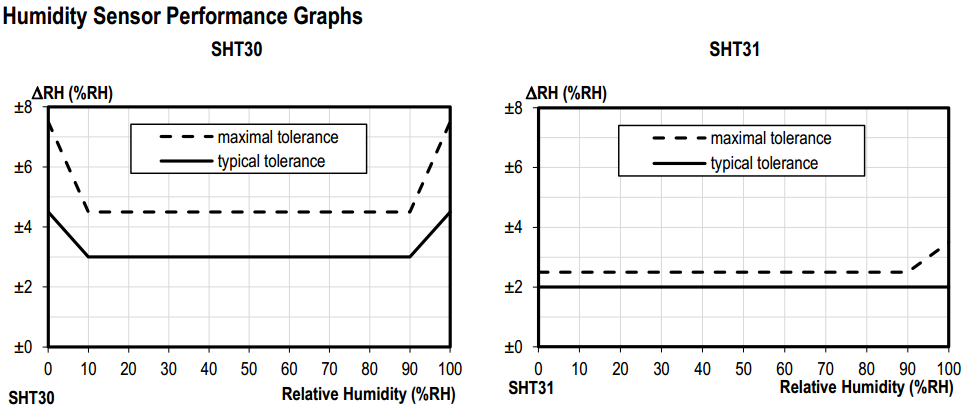
\includegraphics[width=\textwidth]{SHPG.png}
\end{figure}
\begin{figure}[h!]
\centering
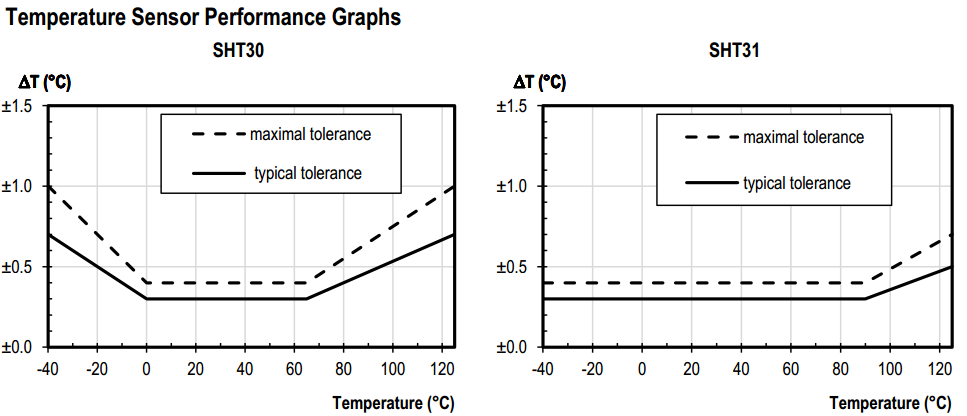
\includegraphics[width=\textwidth]{THPG.png}
\end{figure}


\hfill\subsection{Zapojení modulu}
%naimportuje schema
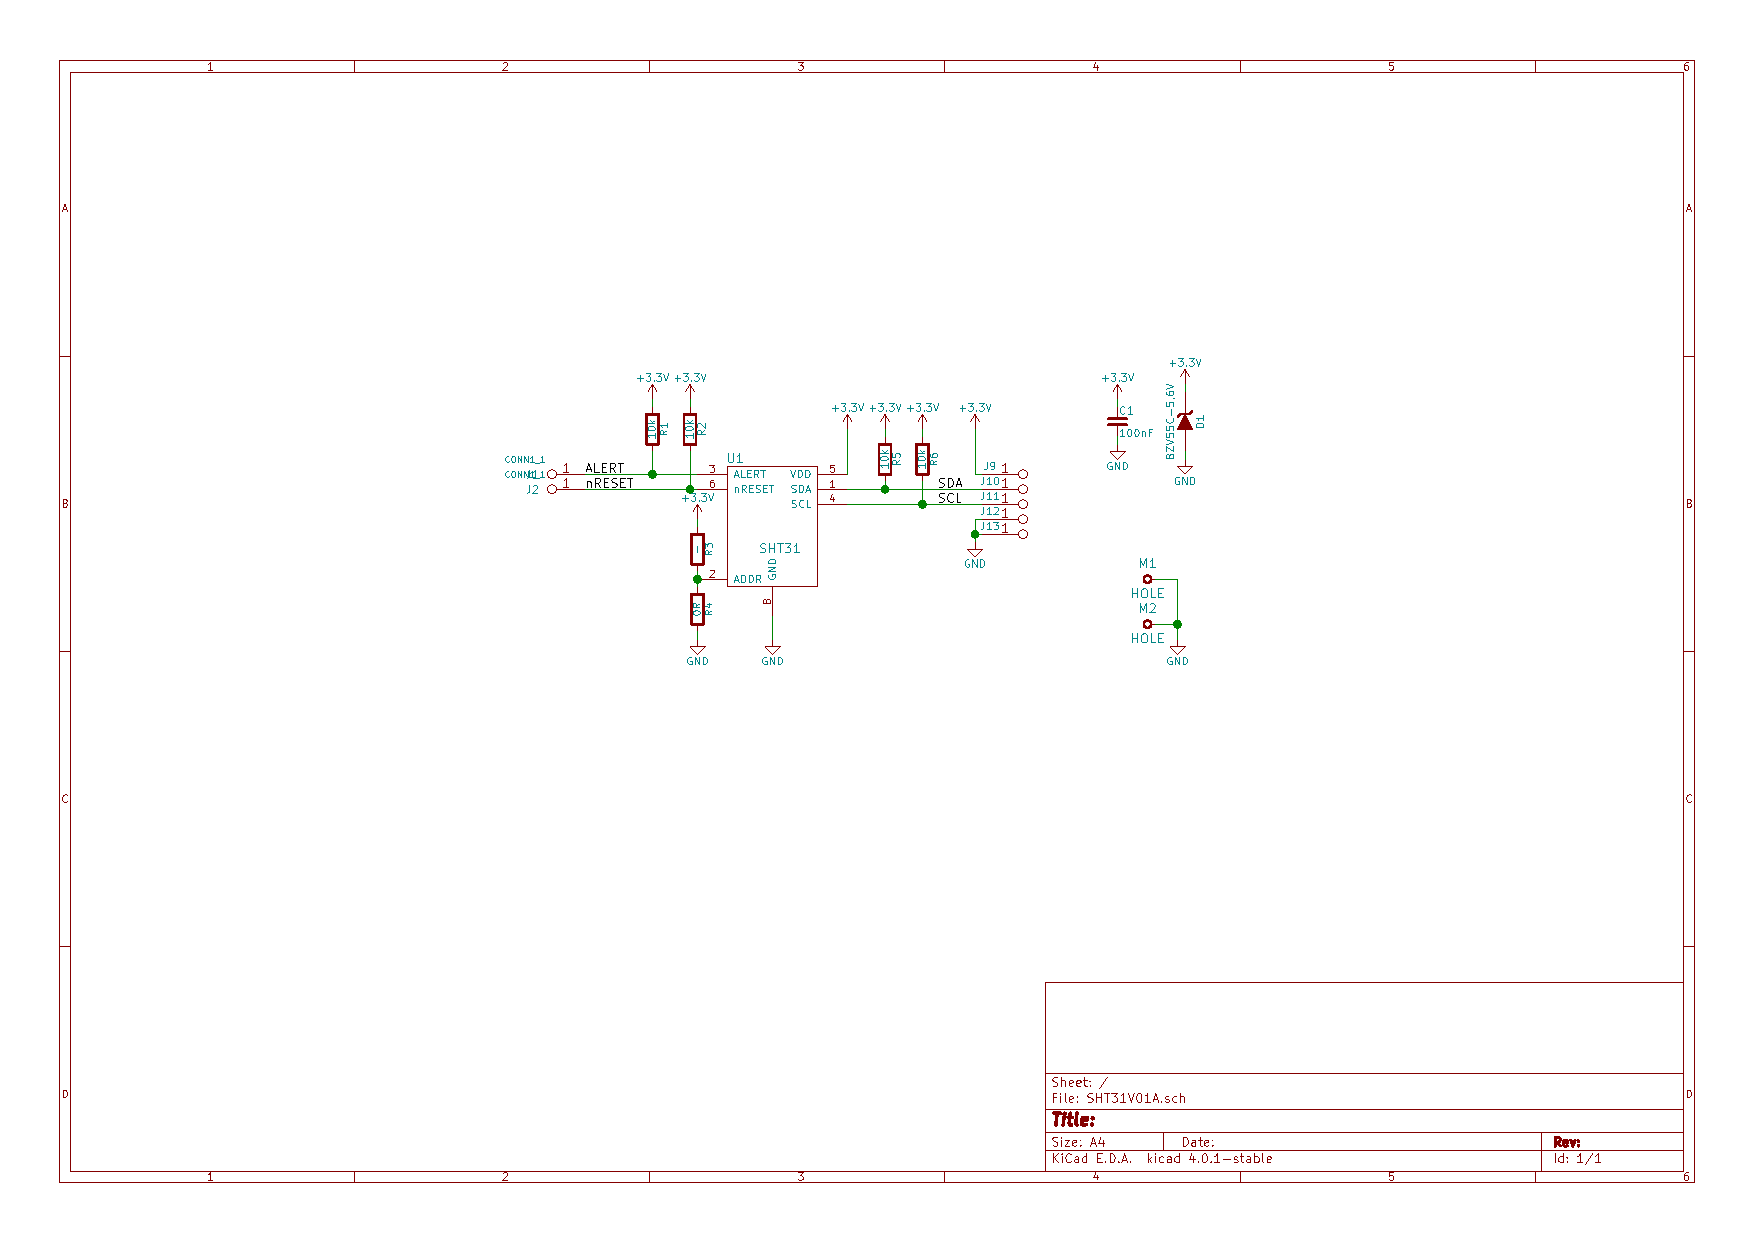
\includepdf[angle=90]{../../hw/sch_pcb/SHT31V01A.pdf}

\section{Osazení a oživení}
% totot naimportuje cast, kde jsou osazováky a BOM tabulka
\subsection{Osazení}


\begin{figure}[ht!]
	\centering
	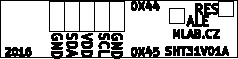
\includegraphics[scale=2]{../../hw/CAM_PROFI/SHT31V01A-top_cropped.pdf}
	\qquad
	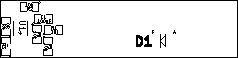
\includegraphics[scale=2]{../../hw/CAM_PROFI/SHT31V01A-bottom_cropped.pdf}
\end{figure}

\begin{center}
  \begin{tabular}{ | l | l | l | l |}
    \hline
    Označení & Hodnota, typ & Pouzdro & Počet \\ \hline
    \hline
			J10, J11, J9, J12, J13 & JUMP\_2x1 & Straight\_1x02 & 5\\ \hline
			D1 & BZV55C-5,6V & Diode-MiniMELF\_Standard & 1\\ \hline
			U1 & SHT31 & DFN-8-1EP\_2.4x2.4mm\_Pitch0.5mm & 1\\ \hline
			J1, J2 & CONN1\_1 & Straight\_1x01 & 2\\ \hline
			R4 & 0R & SMD-0805 & 1\\ \hline
			R5, R6, R1, R2 & 10k & SMD-0805 & 4\\ \hline
			R3 & - & SMD-0805 & 1\\ \hline
			M1, M2 & HOLE & MountingHole\_3mm & 2\\ \hline
			C1 & 100nF & SMD-0805 & 1\\ \hline
	
  \end{tabular}
\end{center}
\subsection{Oživení}
Je potřeba provést kontrolu zda není na plošném spoji zkrat a zda je dobře zapájen IO. Jinak není třeba nic oživovat, pouze připojit a napsat program.

Když je nulovým odporem osazena pozice R4 adresa modulu je 0x44, pokud je osazena pozice R3 je adresa 0x45.
\section{Program}
Vzorový program se nachází ve složce SW modulu. Pro spuštění je potřeba mít nainstalovaný  pyMLAB.

\end{document}
